\documentclass{article}
\usepackage[utf8]{inputenc}
\usepackage{caption}
\usepackage[margin=1in]{geometry}
\usepackage{graphicx}
\usepackage{pdfpages}
\pdfminorversion=7

\begin{document}
\begin{titlepage}


\centering
\vspace*{2cm}
{\Huge System Design Document\par}
\vspace{.25cm}
{\LARGE Course Evaluation System\par}
\vspace{1cm}
{\Large Team EVAL\par}
\vspace{.2cm}
{\Large Jovon Craig, Sam Elliott, Robert Judkins, and Stanley Small\par}
\vspace{1cm}
{\Large Client: Dr. Harlan Onsrud\par}
\vspace{1cm}
{\Large November 16, 2018\par}
\vspace{11cm}

University of Maine - Fall of 2018 - COS 397

Instructor: Professor Terry Yoo

\end{titlepage}

\newpage

\begin{center}
{
\includegraphics[scale=.2]{images/team_logo.png}} \\ 	\bigskip
{\LARGE Course Evaluation System } \\ \medskip
{\large System Design Document } \\ \medskip
\end{center}

\tableofcontents

\newpage

\section{Introduction}
Team EVAL is creating a system to more efficiently create and distribute post-semester teaching evaluations. The system will be built to interface with LimeSurvey, a popular open-source survey application. 

\subsection{Purpose of This Document}

This system design document gives an overview of the structure and planned implementation of our course evaluation system. The first section describes the system architecture, how the components function, and how the components relate to each other. The second section covers the design of the data, detailing the database schema and the properties of the files that are used by the system. The document's third section has a table that lists the components that fulfill each functional requirement.

This document is intended for the development team, the product client, Dr. Harlan Onsrud, and potential users of the system. Team EVAL needs this document to ensure that the product works as intended. Dr. Onsrud needs it to know that the program that he desires will be fully realized. The document also helps the software's users in that they can learn more about the functions and architecture of the evaluation system.

\subsection{References}

Craig, J., Elliott, S., Judkins, R., \& Small, S. 29 October 2018. \textit{System Requirements Specification.}
\vspace{2mm}\newline
Craig, J., Elliott, S., Judkins, R., \& Small, S. 30 November 2018. \textit{User Interface Design Document.}
\vspace{2mm}\newline
Fowler, M. (2004). \textit{UML Distilled: A Brief Guide to the Standard Object Modeling Language.} Boston:

Addison-Wesley.
\vspace{2mm}\newline
Using OAuth 2.0 to Access Google APIs  |  Google Identity Platform  |  Google Developers. Google, Google,

12 Nov. 2018,  \underline{developers.google.com/identity/protocols/OAuth2}.
\vspace{2mm}\newline
Onsrud, H. ``Example Question Selection Form.'' See Appendix D.

\section{System Architecture}
\subsection{Architectural Design}

Figure 1 is a high-level abstraction of the proposed system architecture. With this figure, we aim to communicate what components are in the system and the API allowing the components to communicate.

\begin{center}
\captionof{figure}{Component diagram of the system (left); sequence diagram of  Google OAuth 2.0 (right)}
\vspace{2mm}
\label{fig:componentdiagram}
{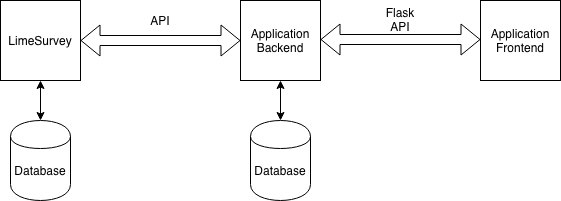
\includegraphics[scale=.55]{images/component_diagram.png}} 
\hspace{2mm}
{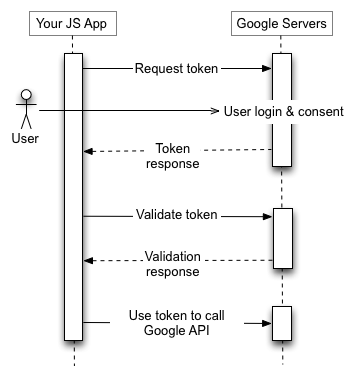
\includegraphics[scale=.5]{images/tokenflow.png}} 
\end{center}

\vspace{3mm}

Figure 2 is a technology architecture diagram that shows the languages and frameworks that the team will use to make the system.

\begin{center}
\captionof{figure}{Technology diagram of the system}
\label{fig:technologydiagram}
{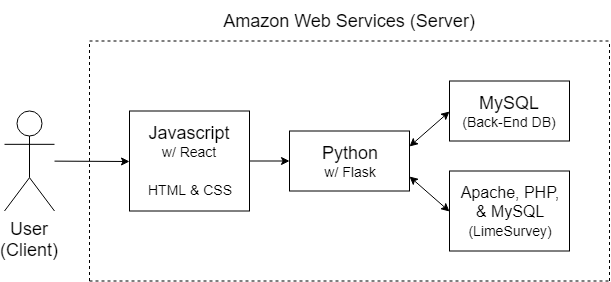
\includegraphics[scale=.6]{images/technology_architecture_diagram.png}} 
\end{center}

LimeSurvey (version 3.15.3+181108) is running on an Apache web server that uses PHP version 5.6. This survey software maintains a database running on MySQL 5.5.61. The team will use Amazon Web Services to host the evaluation system on the Web at \underline{teachingevaluations.org}, providing a scalable solution to fluctuating demand and peak use after the semester.

The system consists of three major components, which communicate via an API. The front end, which handles the user interface, and displays the visuals and data sent from the API. It will be written in JavaScript using the React framework, along with HTML and CSS. The back end communicates with the databases, which are hosted by the same database management system. It will be written in Python, and its endpoints will use the Flask library.  The database stores survey templates and responses using MySQL.

A single API will connect the front end to the back end and the back end to LimeSurvey and our database. A REST interface connects the front end to the back end using endpoints. Separate functions will utilize the LimeSurvey API so that the back end can access the LimeSurvey database.  LimeSurvey is outside the scope of the project and our system will not alter LimeSurvey in any way.  A user will have no contact with LimeSurvey and will only communicate with the front end. 

Google OAuth 2.0 will be used to authenticate users with their Google accounts. Each student at the University of Maine is issued a Google Apps account e-mail which can be used to log in to the teaching evaluation system. As shown in the right side of Figure 1, the application will request a token from Google. The application will then store this token in a cookie. When a page is refreshed, the token is validated on Google's servers. Google OAuth 2.0 can also provide information such as the user's name and e-mail. 

\subsection{Decomposition Description}

Figure 3 abstracts the major functions that are expected to be in the system. This sequence diagram, shown on the next page, illustrates a typical session and is meant to communicate a more detailed view of the components and their relationships. The ``Database'' refers to the database that we will be implementing to store survey templates and responses.

\newpage

\begin{center}
\captionof{figure}{Sequence diagram of an example session}
\label{fig:sequencediagram}
{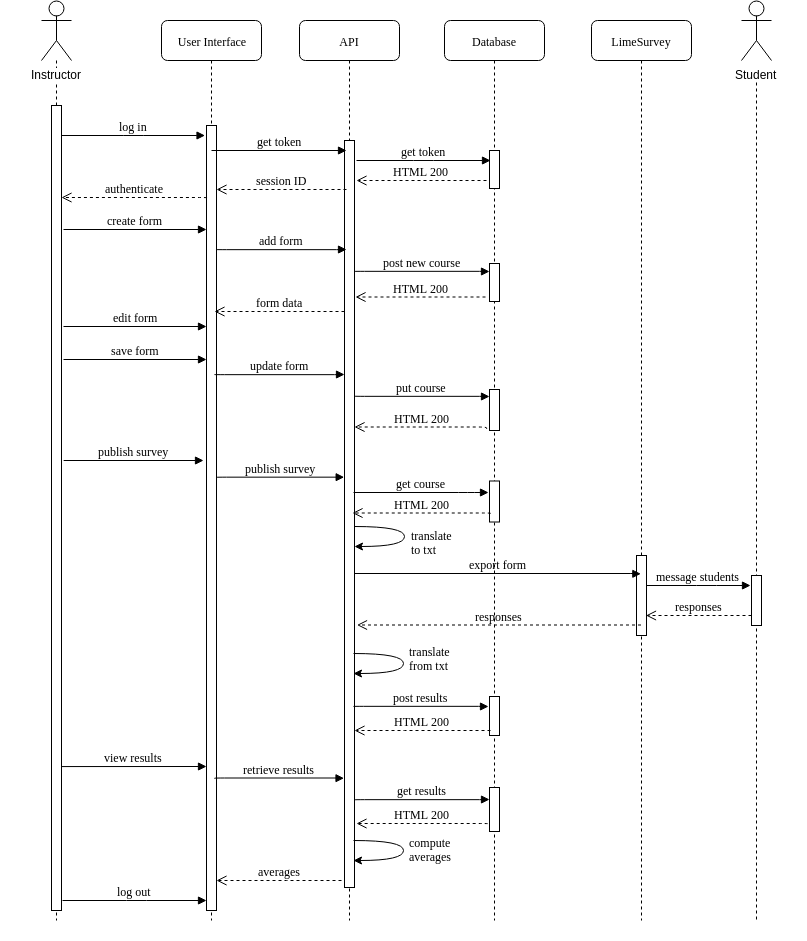
\includegraphics[scale=.55]{images/sequence_diagram.png}}
\end{center}

\newpage

To begin using the course evaluation system, the instructor must first log in with a username and password (``log in''). The API retrieves the user's token from the database to confirm that the password is correct (``get token'', ``authenticate''). Next, the instructor creates an evaluation form to send to students (``create form''). The API adds an empty course to the database (``add form'', ``post new course''). The instructor then edits the survey with the appropriate info and saves the form (``edit form'', ``save form''). Upon saving, the API updates the database with the entered information (``update form'', ``put course'').

With an evaluation form completed, the instructor can then publish it online (``publish survey''). The API retrieves the course information from the database to translate the survey form into a tab-separated .txt file (``get course'', ``translate to txt''). It then sends the .txt file to LimeSurvey and tells the survey software to message the students through e-mail (``export form'', ``message students''). The API retrieves the students' responses, translates them from another tab-separated .txt file, and stores them into the database (``translate from txt'', ``post results''). Finally, the instructor can view the survey results, with the help of the API getting the results from the database and finding their averages (``retrieve results'', ``get results'', ``compute averages'').

\subsubsection{Endpoint Descriptions}

The following table briefly describes the API's endpoints, which query data from the back-end database:

\begin{center}
\captionof{table}{API endpoint descriptions}
\begin{tabular}{|p{2cm}|p{2cm}|p{8cm}|} 
\hline
\textbf{Type} & \textbf{Name} & \textbf{Description} \\
\hline
GET & /login & retrieves a token for a certain authentication key\\ 
\hline
POST & /create\_user & adds a user to the database\\ 
\hline
GET & /courses & retrieves a list of all courses\\ 
\hline
GET & /course & retrieves the info for a given course\\ 
\hline
PUT & /course & updates the info for a given course\\ 
\hline
DELETE & /course & removes a given course\\ 
\hline
POST & /new\_course & creates a new course\\ 
\hline
GET & /results & retrieves a list of survey results for a given course\\ 
\hline
POST & /results & updates a list of survey results for a given course\\ 
\hline
\end{tabular}
\end{center}

\vspace{0mm}

\section{Persistent Data Design}
\subsection{Database Descriptions}

Our database will include tables that store information about courses, survey questions, and survey responses. A diagram of the database schema is shown on the next page:

\vspace{3in}
\begin{center}
\captionof{figure}{Schema diagram of the back-end database}
\label{fig:schemadiagram}
{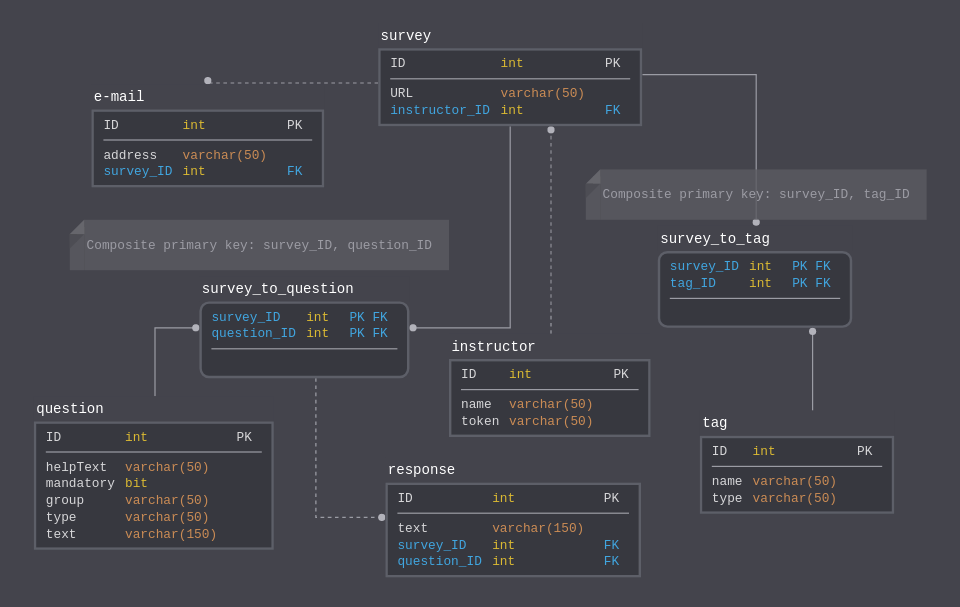
\includegraphics[scale=.6]{images/schema_diagram.png}} 
\end{center}

\vspace{5mm}

The database contains six object tables and two relationship tables. The \textbf{Survey} table contains survey IDs, the surveys' URLs (generated by LimeSurvey) and associated instructor IDs. The e-mail addresses to send the surveys to are stored in the \textbf{E-mail} table. The \textbf{Instructor} table contains the names of the instructors along with authentication tokens generated by Google OAuth. The \textbf{Tag} table contains additional information (e.g. course names) about the surveys. These tags are used to categorize and search surveys. The \textbf{Question} table contains all questions to be entered into the surveys, along with help text and the type of question. The \textbf{Response} table includes students' responses to certain questions. The relationship tables, \textbf{Survey-to-Question} and \textbf{Survey-to-Tag}, link the surveys to their appropriate questions and tags.



\subsection{File Descriptions}

The system requires several pieces of data, including database files, front-end markup, and LimeSurvey files, to run as intended. A file structure diagram is given on the next page:

\newpage
\begin{center}
\captionof{figure}{Diagram of the files used by the system}
\label{fig:filediagram}
{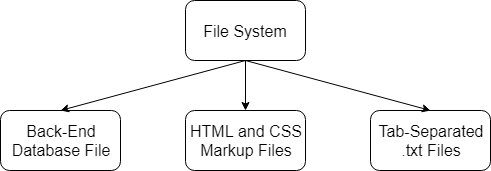
\includegraphics[scale=.64]{images/file_structure_diagram.png}} 
\end{center}

\vspace{3mm}

The back-end database has a file to keep track of all course information, survey forms, and survey responses that users have input. The schema in the previous section shows the fields and types in that file. To reduce the risk of a breach, any survey results in the database get removed by the system 60 days after viewed by the instructor. 

The front end will be implemented in JavaScript, so our file structure will include .js files that operate the front end. There are also mark-up files, which specify the look and feel of the front end. The back-end will be implemented in Python and our file structure will include .py files that operate the back end. The JavaScript and Python files are static and permanent, and thus do not require maintenance.

Lastly, the system briefly stores LimeSurvey files in the form of tab-separated text documents. They either contain survey form data or student responses. The form data files are deleted immediately after they are sent to LimeSurvey, and the response data files are deleted immediately after they are stored in the database.

\section{Requirements Matrix}

The following table lists the functions in our system, as shown in the sequence diagram, that meet each functional requirement given in the system requirements specification:

\begin{center}
\captionof{table}{Requirements matrix}
\begin{tabular}{|p{3.2cm}|p{3.2cm}|p{6cm}|} 
\hline
\textbf{Use Case Number} & \textbf{Use Case Name} & \textbf{System Component(s)} \\
\hline
1 & Log on & log in, get token\\ 
\hline
2 & Create survey & create form, add form, post new course\\ 
\hline
3 & Edit survey & edit form, save form, update form, put course\\ 
\hline
4 & Publish survey & publish survey, get course, translate to txt, export form, message students\\ 
\hline
5 & View survey results & view results, retrieve results, get results, compute averages\\ 
\hline
\end{tabular}
\end{center}

\appendix

\newpage
\section{Agreement Between Customer and Contractor}
This page shows that all members of Team EVAL and the client, Harlan Onsrud, have agreed on all the information in the system design document. By signing this document, Team EVAL and Dr. Onsrud agree on the system's architecture, components, relations between the components, database schema, required files, and file descriptions.

The team will follow a process in the case that the design document is changed after we sign it. First, the team writes a rough draft of the changes to be made to the document. Second, all team members and Harlan Onsrud will sign the document agreeing to the changes. Finally, the changes are made to the final copy of the document.

\vspace{.7in}
\noindent
\begin{tabular}{ p{5cm} p{5cm} p{5cm} } 
\textbf{\textit{Name}} & \textbf{\textit{Signature}} & \textbf{\textit{Date}} \\[.5cm]
\textbf{Jovon Craig} & $\rule{5cm}{.1mm}$ & $\rule{5cm}{.1mm}$\\[.5cm]
\textbf{Sam Elliott} & $\rule{5cm}{.1mm}$ & $\rule{5cm}{.1mm}$\\[.5cm]
\textbf{Robert Judkins} & $\rule{5cm}{.1mm}$ & $\rule{5cm}{.1mm}$\\[.5cm]
\textbf{Stanley Small} & $\rule{5cm}{.1mm}$ & $\rule{5cm}{.1mm}$\\[.5cm]
\textbf{Harlan Onsrud} & $\rule{5cm}{.1mm}$ & $\rule{5cm}{.1mm}$\\[.5cm]
Customer Comments: & \multicolumn{2}{ l }{ $\rule{10.45cm}{.1mm}$ }\\[.5cm]
\multicolumn{3}{ l }{ $\rule{15.9cm}{.1mm}$ }\\[.5cm]
\end{tabular}

\newpage
\section{Team Review Sign-off}

This page shows that all members of Team EVAL have reviewed the system design document and agreed on its content. By signing this document, the team members agree on that all information about the system's architecture and design are accurate. There is nothing in the document that is a source of contention.

\vspace{.7in}
\noindent
\begin{tabular}{ p{5cm} p{5cm} p{5cm} } 
\textbf{\textit{Name}} & \textbf{\textit{Signature}} & \textbf{\textit{Date}} \\[.5cm]
\textbf{Jovon Craig} & $\rule{5cm}{.1mm}$ & $\rule{5cm}{.1mm}$\\[.5cm]
Comments: & \multicolumn{2}{ l }{ $\rule{10.45cm}{.1mm}$ }\\[.5cm]
\multicolumn{3}{ l }{ $\rule{15.9cm}{.1mm}$ }\\[.5cm]
\textbf{Sam Elliott} & $\rule{5cm}{.1mm}$ & $\rule{5cm}{.1mm}$\\[.5cm]
Comments: & \multicolumn{2}{ l }{ $\rule{10.45cm}{.1mm}$ }\\[.5cm]
\multicolumn{3}{ l }{ $\rule{15.9cm}{.1mm}$ }\\[.5cm]
\textbf{Robert Judkins} & $\rule{5cm}{.1mm}$ & $\rule{5cm}{.1mm}$\\[.5cm]
Comments: & \multicolumn{2}{ l }{ $\rule{10.45cm}{.1mm}$ }\\[.5cm]
\multicolumn{3}{ l }{ $\rule{15.9cm}{.1mm}$ }\\[.5cm]
\textbf{Stanley Small} & $\rule{5cm}{.1mm}$ & $\rule{5cm}{.1mm}$\\[.5cm]
Comments: & \multicolumn{2}{ l }{ $\rule{10.45cm}{.1mm}$ }\\[.5cm]
\multicolumn{3}{ l }{ $\rule{15.9cm}{.1mm}$ }\\[.5cm]
\end{tabular}


\newpage
\section{Document Contributions}

Stanley Small included a template of the appendices and he wrote a draft of the title page, architectural design section, and database description. He also added the component diagram along with the Google OAuth sequence diagram, and helped with the database schema. Stan contributed approximately 30 percent of the document.


Jovon Craig wrote the purpose of the document, references, decomposition description, file descriptions, and requirements matrix. He made revisions to the title page, architectural design section, and database description. He also added the sequence diagram and file diagram, revised the technology diagram, and made a draft of the database schema. Jovon contributed about 40 percent of the document.


Sam Elliott created the technology diagram rough draft, and made revisions to the sequence diagram and the file diagram and added many of them to the document. He revised the architecture design section and the file descriptions section, as well as general changes based on feedback from the SRS and Dr. Onsrud.  He was the main point of contact with Dr. Onsrud for reviewing the document and organizing meetings. Sam contributed about 20 percent of the document.

Robert Judkins converted the document to LaTeX and helped with front-end design. Robert contributed about 10 percent of the document.

\newpage

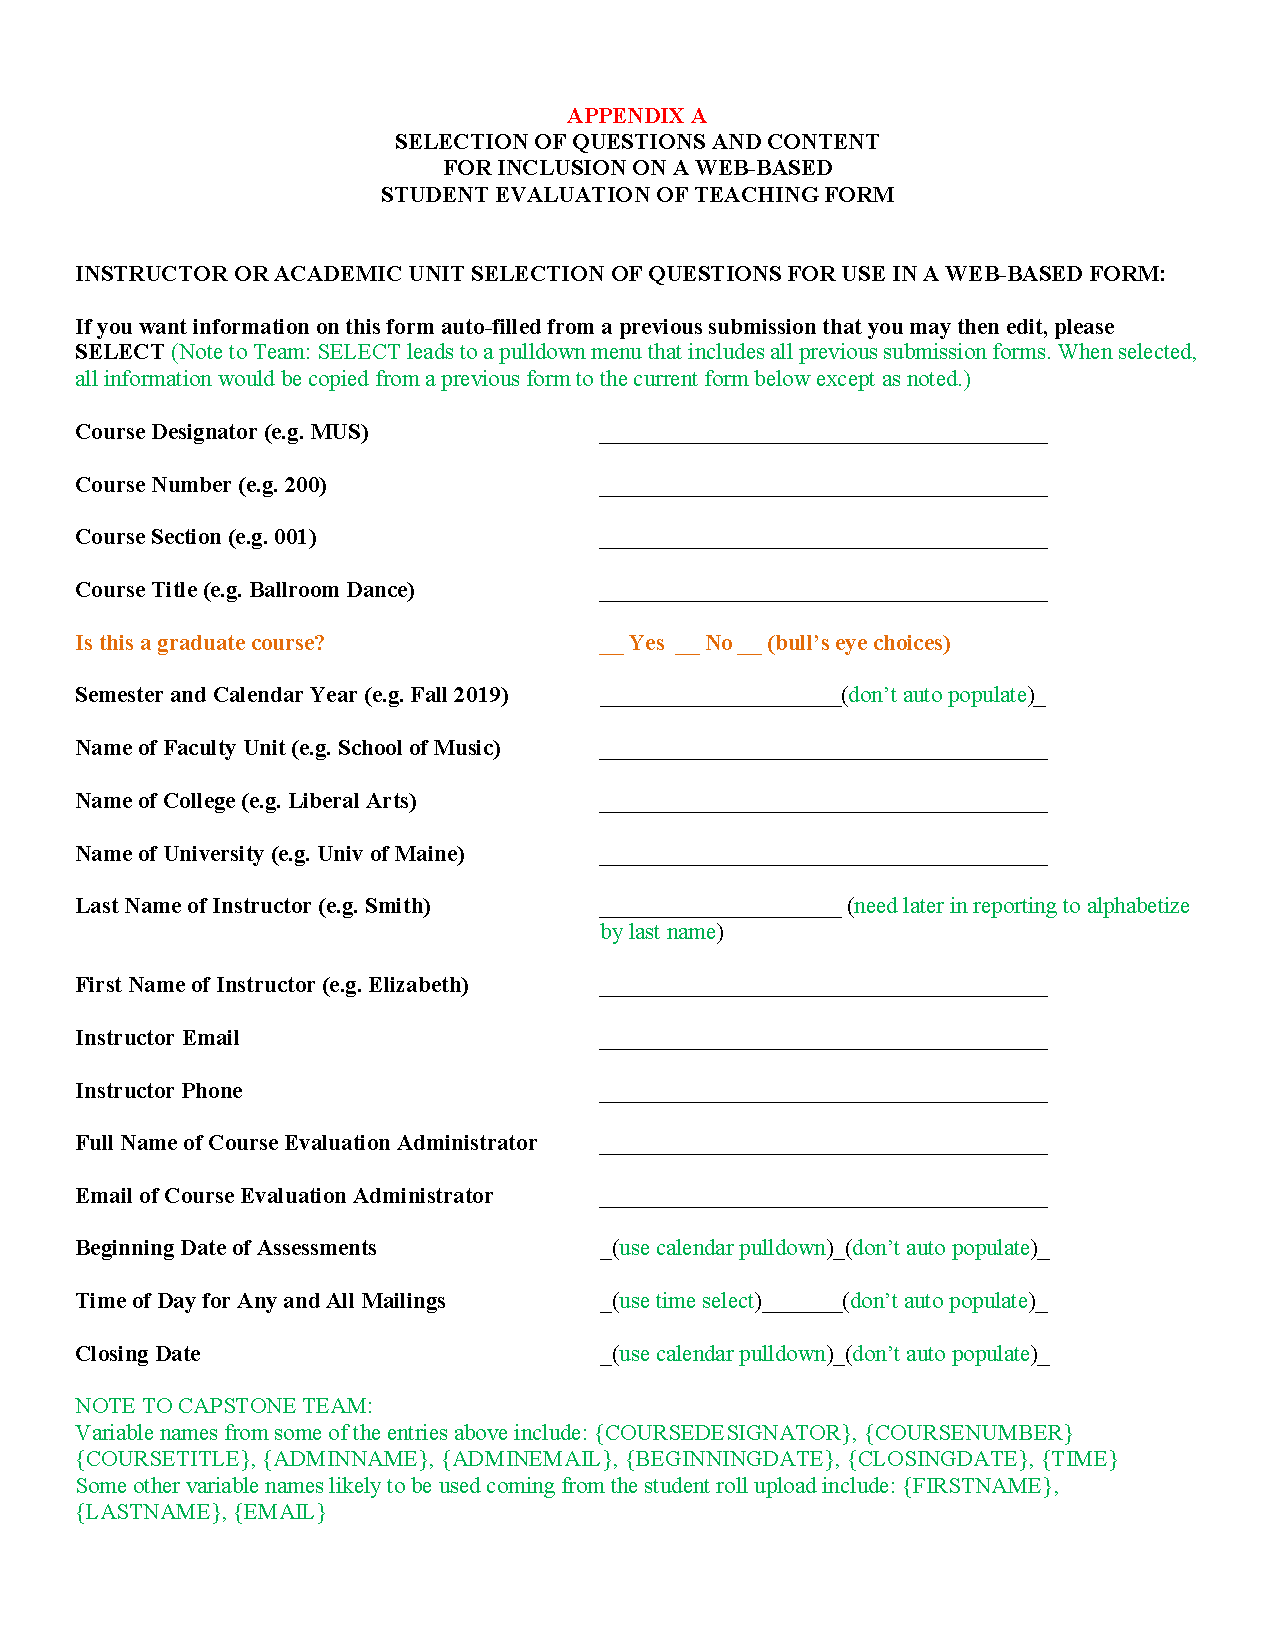
\includepdf[scale=0.85,pages=1,pagecommand=\section{Example Question Selection Form}]{images/question_appendix.pdf}
\includepdf[scale=0.85,pages=2-]{images/question_appendix.pdf}

\end{document}
